\section{Background}\label{sec:ch6:background}
\subsection{Related Work}\label{sec:ch6:related} 
Fujieda et.\ al.\ use a DWT in combination with a
CNN to do texture classification and image annotation 
\cite{fujieda_wavelet_2017, fujieda_wavelet_2018}. They take a
multiscale wavelet transform of the input image, combine the activations at each
scale independently with learned weights, and feed these back into the network
at locations where the activation resolution matches the subband resolution. The
architecture block diagram is shown in \autoref{fig:ch6:fujieda}, taken from the
original paper. They found that their `Wavelet-CNN' could
outperform competitive non-wavelet-based CNNs on both texture classification and
image annotation.

\begin{figure}[bt]
  \centering
  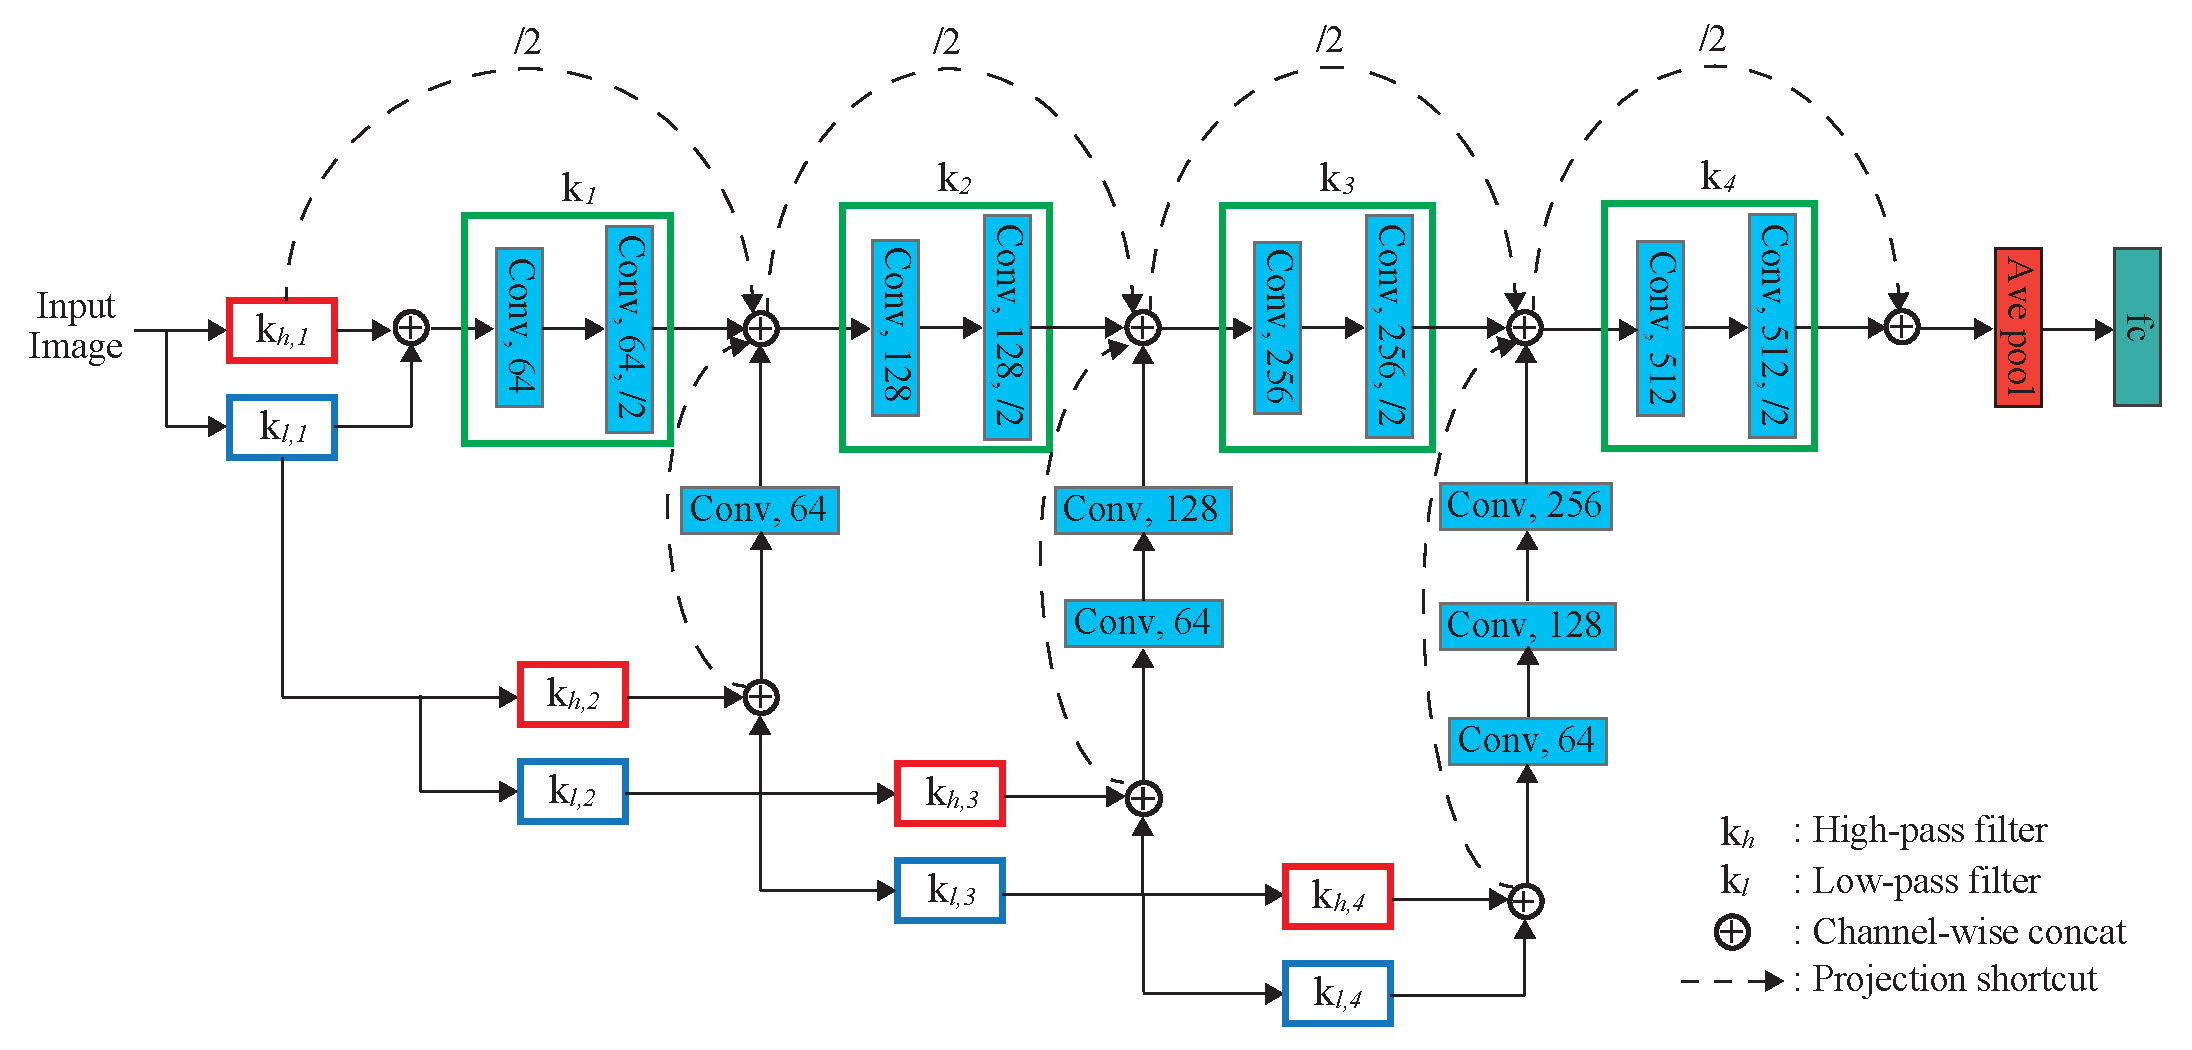
\includegraphics[width=\textwidth]{\imgpath/wavelet_CNN_3.pdf}
  \mycaption{Architecture using the DWT as a frontend to a CNN}{Figure 1 from
  \cite{fujieda_wavelet_2018}. Fujieda et.\ al.\ take a multiscale wavelet
  decomposition of the input before passing the input through a standard
  CNN\@. They learn convolutional layers independently on each subband and feed
  these back into the network at different depths, where the resolution of the
  subband and the network activations match.}
  \label{fig:ch6:fujieda}
\end{figure}

Several works also use wavelets in deep neural networks for super-resolution
\cite{guo_deep_2017} and for adding detail back into dense pixel-wise
segmentation tasks \cite{ma_detailed_2018}. These typically save wavelet
coefficients and use them for the reconstruction phase.

In \cite{rippel_spectral_2015}, \citeauthor{rippel_spectral_2015}
parameterize filters in the DFT domain. Rather than having a pixel domain filter
$w \in \reals[F\x C\x K\x K]$, they learn a set of Fourier coefficients
$\hat{w} \in \complexes[F\x C\x K \x \ceil{K/2}]$
(the reduced spatial size is a result of enforcing that the inverse DFT of their
filter to be real, so the parameterization is symmetric). On the forward pass of
the neural network, they take the inverse DFT of $\hat{w}$ to obtain
$w$ and then convolve this with the input $x$ as a normal CNN
would do\footnote{The convolution may be done by taking both the image and
filter back into the Fourier space but this is typically decided by the
framework, which selects the optimal convolution strategy for the filter and
input size. Note that there is not necessarily a saving to be gained by
enforcing it to do convolution by product of FFTs, as the FFT size needed for
the filter will likely be larger than $K\x K$, which would require resampling
the coefficients.}. 

Note that an important point should be emphasized about reparameterizing filters
in either the wavelet or Fourier domains: many invertible linear
transform of the parameter space will not change parameter updates if a linear
optimization scheme is used (for example standard GD, or SGD with momentum). 
\citeauthor{rippel_spectral_2015}
mention in their work that this holds for \emph{all} invertible
transforms but this is not strictly true, and we prove in
\autoref{appC:invertible} that it only holds for \emph{tight frames}. 
We make this point clear as a natural extension to continue the work
in \cite{rippel_spectral_2015} would be to parameterize filters in the \emph{wavelet} domain,
taking inverse transforms and then doing normal convolution. 

While \cite{rippel_spectral_2015} was an inspiration for this chapter, the work we
present here is not a reparameterization in the wavelet domain with convolution
in the pixel domain. Instead, we learn wavelet filters \emph{and} perform filtering in the wavelet domain too.

\subsection{Notation}
We make use of the 2-D $Z$-transform to simplify our analysis:
%
\begin{equation}
  X(\zz) = \sum_{n_1}\sum_{n_2} x[n_1, n_2]z_1^{-n_1}z_2^{-n_2} =
  \sum_{\nn}x[\nn]\zz^{-\nn}
\end{equation}
%
As we are working with three-dimensional and four-dimensional arrays but are
only doing convolution in two, we introduce a slightly modified 2-D $Z$-transform
which includes the channel index $c$ and the filter number $f$:
\begin{align}
  X(c, \zz) & = \sum_{n_1}\sum_{n_2} x[c, n_1, n_2]z_1^{-n_1}z_2^{-n_2} =
    \sum_{\nn}x[c, \nn]\zz^{-\nn} \label{eq:ch6:ztransform} \\
  H(f, c, \zz) & = \sum_{n_1}\sum_{n_2} h[f, c, n_1, n_2]z_1^{-n_1}z_2^{-n_2} =
    \sum_{\nn}h[f, c, \nn]\zz^{-\nn} \label{eq:ch6:ztransform2}
\end{align}
We then define the product of these new $Z$-transform signals to be the
channel-wise convolution. E.g. for the 4-D filter $h[f, c, \nn]$ with $Z$-transform
$H(f, c, \zz)$ and the the 3-D signal $x[c, \nn]$ with $Z$-transform $X(c, \zz)$,
let us call the product of the two $Z$-transforms:
\begin{equation}
  X(c, \zz)H(f, c, \zz) = \sum_{\nn}\left(\sum_{\bmu{k}}h[f, c, \nn-\bmu{k}]x[c, \bmu{k}]\right)\zz^{-\nn} \label{eq:ch6:zproduct}
\end{equation}
%
Recall from \autoref{sec:ch2:conv_layers} that a typical convolutional
layer in a standard CNN gets the next layer's output in a two-step process:
%
\begin{align} 
  \cnndlact{y}{l+1}{f}{\nn} &= \sum_{c=0}^{C_l - 1} \cnndlact{x}{l}{c}{\nn} \conv h^{(l)}[f, c, \nn]
    \label{eq:ch6:conv}\\
    \cnndlact{x}{l+1}{f}{\nn} & =  \sigma \left( \cnndlact{y}{l+1}{f}{\nn} \right) \label{eq:ch6:nonlin}
\end{align}
%
If we define the nonlinearity $\sigma_z$ to be the action of $\sigma$ to each
$z$-coefficient in the polynomial $Y(f, \zz)$, then we can rewrite
\eqref{eq:ch6:conv} and \eqref{eq:ch6:nonlin} as:
%
\begin{align}
  \cnnlact{Y}{l+1}{f}{\zz} &= \sum_{c=0}^{C_l - 1} \cnnlact{X}{l}{c}{\zz} H^{(l)}(f, c, \zz) \\
  \cnnlact{X}{l+1}{f}{\zz} &= \sigma_z(\cnnlact{Y}{l+1}{f}{\zz})
\end{align}
%
\subsection{$\DTCWT$ Notation}
For this chapter, we will work with lots of $\DTCWT$ coefficients so we define
some slightly new notation here.

A $J$ scale 2-D $\DTCWT$ gives $6J+1$ coefficients, 6 sets of complex
bandpass coefficients for each scale (representing the oriented bands from 15 to 165
degrees) and 1 set of real lowpass ($lp$) coefficients. 
\begin{equation}
  \DTCWT_J(x) = \{ u_{lp}, u_{j,k} \}_{1\leq j\leq J, 0\leq k < 6}
  \label{eq:ch6:dtcwt_coeffs}
\end{equation}

Each of these coefficients has size:
%
\begin{eqnarray}
  u_{lp} &\in & \reals[N\x C\x \frac{H}{2^{J-1}} \x \frac{W}{2^{J-1}}] \\
  u_{j,k} &\in & \complexes[N\x C\x \frac{H}{2^{J}}\x \frac{W}{2^{J}}]
\end{eqnarray}
%
Recall that the lowpass coefficients are twice as large as in a fully decimated
transform due to the interleaving of the four lowpass terms in \autoref{alg:ch3:dtcwt}.

If we ever want to refer to all the subbands at a given scale, we will
drop the $k$ subscript and call them $u_j$. Likewise, $u$ refers to the whole
set of $\DTCWT$ coefficients.

\subsection{Learning in Multiple Spaces}\label{sec:ch6:learning}

\begin{figure}[t]
  \centering
  \subfloat[A regular convolutional layer]{
  \includegraphics[width=0.8\textwidth]{\imgpath/fwd_chaina.pdf}
  }\\
  \subfloat[Gain applied in the wavelet domain]{
  \includegraphics[width=0.8\textwidth]{\imgpath/fwd_chainb.pdf}
  }\\
  \subfloat[Gain and nonlinearity applied in the wavelet domain]{
  \includegraphics[width=0.8\textwidth]{\imgpath/fwd_chainc.pdf}
  }
  % \includegraphics[width=0.8\textwidth]{\imgpath/fwd_chain.jpg}
  \mycaption{Proposed new forward pass in the wavelet domain}{Two network 
  layers with some possible options for processing. Solid lines denote the
  evaluation path and dashed lines indicate relationships. In (a) we see a
  regular convolutional neural network. We have included the dashed lines to
  make clear what we are denoting as $u$ and $v$ with respect to their
  equivalents $x$ and $y$. In (b) we get to $y^{(2)}$ through a different path.
  First, we take the wavelet transform of $x^{(1)}$ to give $u^{(1)}$, apply a
  wavelet gain layer $G^{(1)}$, and take the inverse wavelet transform
  to give $y^{(2)}$. The dotted line for $H^{(1)}$ indicates that this
  path is no longer present. Note that there may not be any possible
  $G^{(1)}$ to make $y^{(2)}$ from (b) equal $y^{(2)}$ from (a). In
  (c) we have stayed in the wavelet domain longer and applied a wavelet
  nonlinearity $\sigma_w$ to give $u^{(2)}$. We then return to the pixel domain
  to give $x^{(2)}$ and continue on from there in the pixel domain.}
  \label{fig:ch6:fwd_chain}
\end{figure}
At the beginning of each layer $l$ of a neural network, we have the activations
$x^{(l)}$. Naturally, all of these activations have their equivalent wavelet
coefficients $u^{(l)}$. 

From \eqref{eq:ch6:conv}, convolutional layers also have intermediate
activations $y^{(l)}$. Let us discern these from the $x$ coefficients and
modify \eqref{eq:ch6:dtcwt_coeffs} to say the $\DTCWT$ of $y^{(l)}$ gives
$v^{(l)}$.

We now propose the \emph{wavelet gain layer} $G$.
% The name `gain layer' comes from the inspiration for this chapter's work, as it
% appears often the first layer of a CNN could be achieved by simply setting gains
% for different regions in the frequency space of an image. 
The gain layer $G$ can be used instead of a convolutional layer. 
It is designed to work on the wavelet coefficients of an activation $u$,
to give wavelet domain outputs $v$. 

This can be seen as breaking the convolutional path in
\autoref{fig:ch6:fwd_chain} and taking a new route to get the next layer's
coefficients. From here, we can return to the pixel domain by taking the
corresponding inverse wavelet transform $\mathcal{W}^{-1}$. Alternatively, we
can stay in the wavelet domain and apply wavelet-based nonlinearities,
$\sigma_{lp}$ and $\sigma_{bp}$ for the lowpass and highpass coefficients
respectively, to give $u^{(l+1)}$. 

Ultimately we would like to explore architecture design with arbitrary sections
in the wavelet and pixel domain, but to do this we must first explore: 
% \begin{enumerate}[itemsep=5pt,parsep=5pt,topsep=0pt]
  % \item \textbf{How effective is a wavelet gain layer $G$ at replacing a
    % standard convolutional layer $H$?}
  % \item \textbf{What are effective wavelet nonlinearities $\sigma_{lp}$ and $\sigma_{bp}$?}
% \end{enumerate}

\begin{enumerate}
  \item \textbf{How effective is a wavelet gain layer $G$ at replacing a
    standard convolutional layer $H$?}
  \item \textbf{What are effective wavelet nonlinearities $\sigma_{lp}$ and $\sigma_{bp}$?}
\end{enumerate}
